In this section, the implementation of converting Canvas to a storable data with JSON format is introduced. Afterwards, a drawing tool which provides user interfaces to draw various elements on Canvas is implemented.

\subsection{Objectified Canvas}

\subsubsection{Fabric.js}
Fabric.js\footnote{http://fabricjs.com/ - accessed 18 July 2016} is a powerful and simple Javascript HTML5 canvas library, which provides interactive object models on top of canvas element. Since native Canvas only provides low-level APIs for creating elements, but not maintains the life cycle of elements on itself. Fabric.js solves this problem with objectifying native elements and encapsulating native methods for drawing elements. 

Instead of dealing with low-level APIs natively provided by Canvas, Fabric.js provides objectified model for elements with different shapes  on top of native methods. It takes charge of canvas state and rendering, make it possible to manipulate objects directly.


\subsubsection{Serialized Canvas}
Since all elements on the Canvas drawn by Fabric.js can are maintained as an object with properties like position, size and styles.
So the Canvas within Fabric.js can be simply serialized to a JSON object or other formats. 

Fabric.js provides a helper function called \textit{toJSON()}, which will serialized the canvas with canvas properties as well as all object models on the canvas. Code list \ref{list:serialized-canvas-imp} is an example that shows how the serialized output looks like if an rectangle object is created by using Fabric.js.

\begin{lstlisting}[language=JavaScript, caption=Serialized Canvas by Fabric.js , label={list:serialized-canvas-imp}]
var canvas = new fabric.Canvas();
canvas.backgroundColor = 'red';
canvas.add(new fabric.Rect({
  left: 50,
  top: 50,
  height: 20,
  width: 20,
  fill: 'green'
}));
console.log(JSON.stringify(canvas));
/* --- Output of serialized Canvas --- 
{"objects":[{"type":"rect","left":50,"top":50,"width":20,"height":20,"fill":"green","overlayFill":null,"stroke":null,"strokeWidth":1,"strokeDashArray":null,"scaleX":1,"scaleY":1,"angle":0,"flipX":false,"flipY":false,"opacity":1,"selectable":true,"hasControls":true,"hasBorders":true,"hasRotatingPoint":false,"transparentCorners":true,"perPixelTargetFind":false,"rx":0,"ry":0}],"background":"rgba(0, 0, 0, 0)"}
*/
\end{lstlisting}

Comparing with output generated by native Canvas mentioned in section \ref{sec:graphical-data-serialization-concept}, this serialized JSON object is not only efficient for storing, but also has the possibility for restoring all object models and re-rendering them on Canvas.

\subsection{Drawing Tool}
The drawing tool is developed on top of the library Fabric.js. It provides the functionalities such as drawing, styling, dragging and resizing of various element. Not only graphical elements, texts could also be rendered and styled on the Canvas while using drawing tool.

Figure \ref{fig:drawing-tool-arch-imp} illustrates an overview of the drawing tool's architecture. 

\begin{figure}[!htbp]
  \centering
    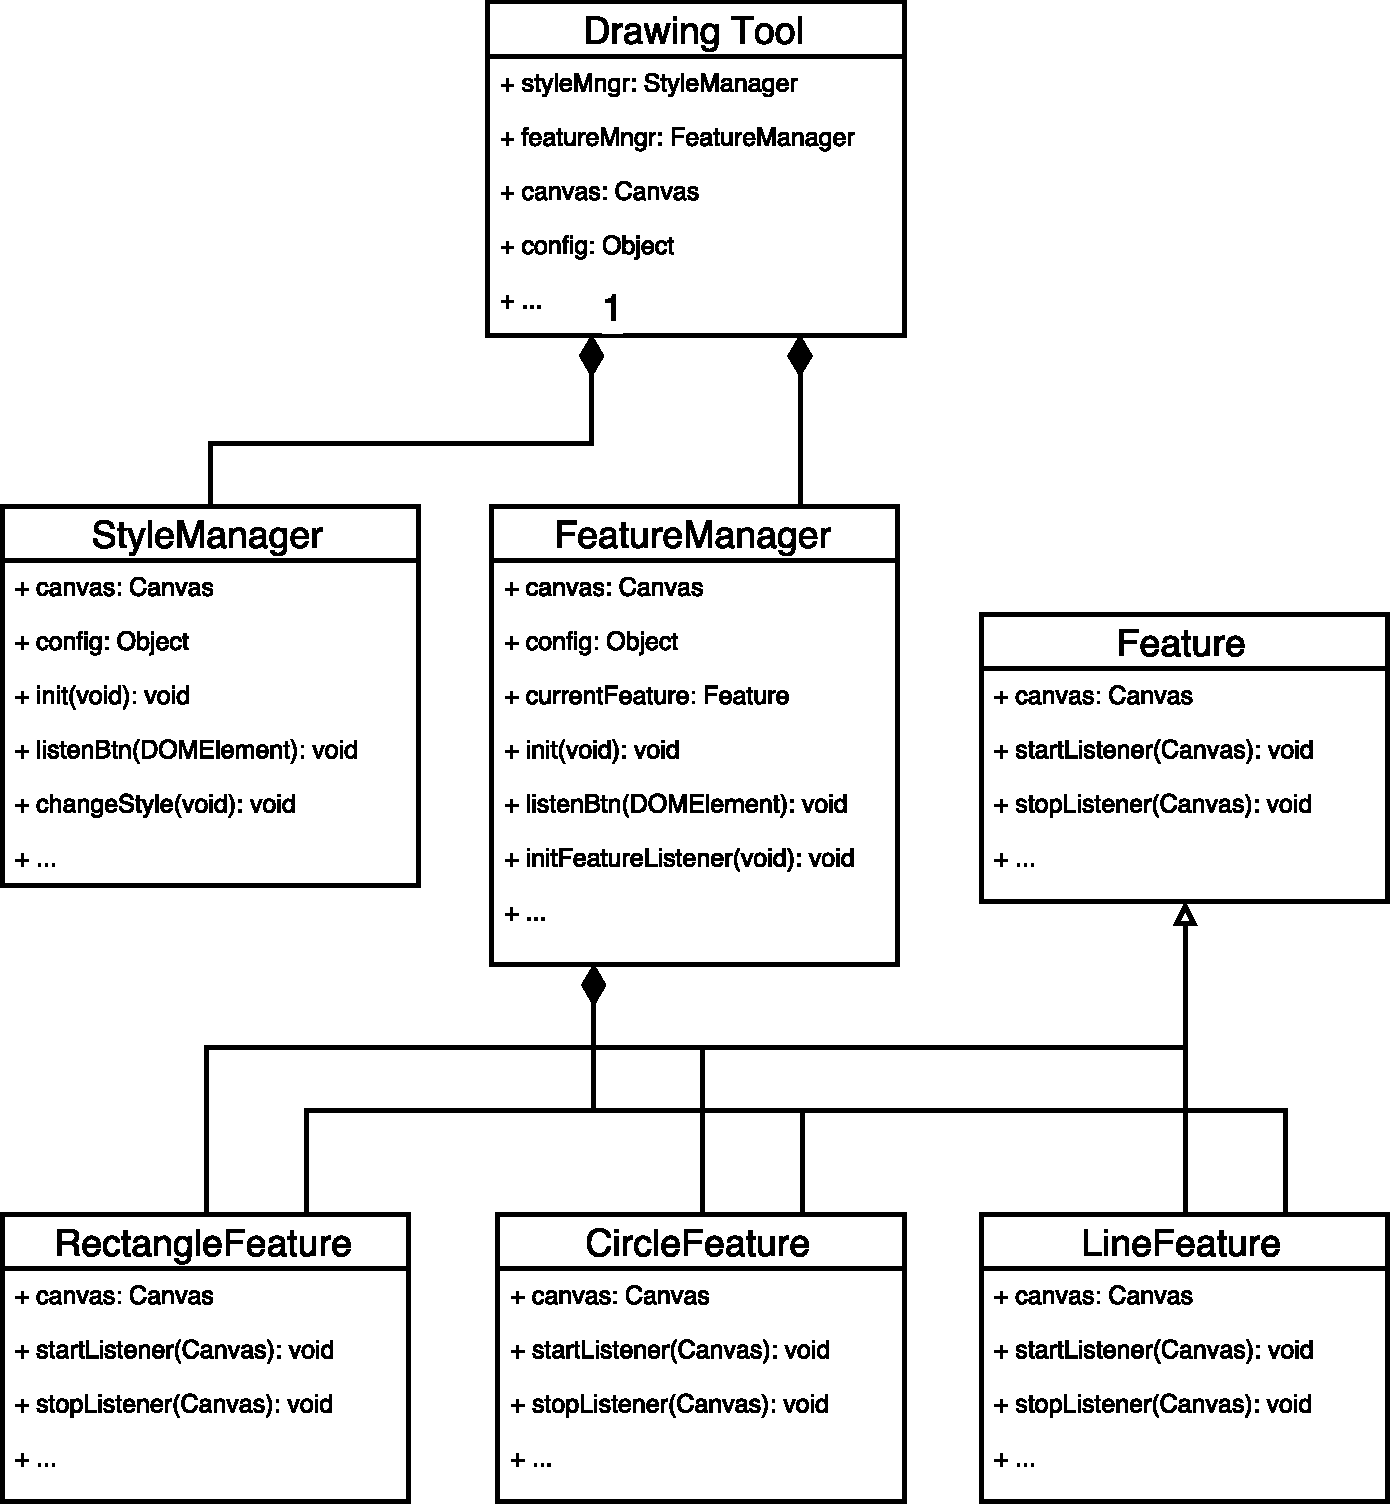
\includegraphics[width=1\textwidth]{Figures/imp-drawing-tool-arch.pdf}
  \caption{Architecture of drawing tool}
  \label{fig:drawing-tool-arch-imp}
\end{figure}

\subsubsection{Style Manager}
At the startup of drawing tool, \textit{StyleManager} is instantiated. \textit{StyleManager} receives the the config instance, in which the DOM elements with relevant styling functionalities are defined. And in the \textit{init()} function of \textit{StyleManager}, listeners for the DOM elements are created. If the DOM elements are triggered by user, \textit{StyleManager} will apply the chosen style to the active objects on the Canvas.

Code list \ref{list:style-manager-imp} takes the listener for DOM element of color picker, which is used for changing the color of a object on Canvas. It acquires the reference of color picker DOM from the config instance, and starts listening for the \textit{onchange} event. If the \textit{onchange} event is fired, the listener will set the object's \textit{fill} property to the color value. Afterwards, the canvas is re-rendered and the active object with new color is shown up.

\begin{lstlisting}[language=JavaScript, caption=Main process of StyleManager, label={list:style-manager-imp}]
class StyleManager {
  constructor(canvas, config){
    this._canvas = canvas;
    this._config = config;
  }
  init(){
    el = this._config['color-picker-dom']
    this._listenColor(el)
    // ... more styling listeners
  }
  _listenColor(el){
    let self = this;
    el.onchange = function(){
      var obj = self.canvas.getActiveObject();
      self._setObjStyle(obj, 'fill', el.value);
      canvas.renderAll();
    }
  }
  // ...
}
\end{lstlisting}


\subsubsection{Feature Manager \& Extensible Features}

In addition, a \textit{FeatureManager} is also created for managing different drawing functionalities. The basic idea of \textit{FeatureManager} is quite similar as \textit{StyleManager} mentioned above. It also listens for the DOM elements to toggle different drawing behaviours.

After that a specific drawing mode is triggered by user, \textit{FeatureManager} will assign listeners for specific mouse events on the Canvas and track the drawing behaviours. According to the mouse events triggered by user on the Canvas, the correlate objects will be rendered into the Canvas context.

\begin{lstlisting}[language=JavaScript, caption=Main process of FeatureManager, label={list:feature-manager-imp}]
class FeatureManager {
  constructor(canvas, config){
    this._canvas = canvas;
    this._config = config;
  }
  init(){
    el = this._config['text-feature-dom']
    this._listenText(el)
    // ... more features' listeners
  }
  _listenText(el){
    let textFeature = new TextFeature(this._canvas);
    el.onclick = (e) => { 
      this._clickHandler(text)
    }
  }
  // ...
}
class TextFeature{
  constructor(canvas){
    this._canvas = canvas;
  }
  startListen(){
    // tracking mouse event
  }
  stopListen(){
    // remove listeners
  }
}
\end{lstlisting}

Features, namely drawing modes are highly extensible on the drawing tool. \textit{TextFeature} in code list \ref{list:feature-manager-imp} is an example. All feature classes need to implement two interfaces \textit{startListen()} and \textit{stopListen()} basically. In \textit{startListen()}, listeners for tracking mouse events are defined. And in \textit{stopListen()}, all listeners should be removed. Both function will called by \textit{FeatureManager} when this drawing mode is toggled.